\documentclass{beamer}

\usepackage[english]{babel}
\usepackage[utf8x]{inputenc}

\usepackage{graphicx}
\graphicspath{ {Images/} }

\title{Plant-Id Requirements and Design}
\author{by Group 3 - Plant-Id \\* Ethan Ahuja - ahujae \\* Ethan Patterson - patteret \\* James Barry - barryj \\* Evan Brass - brassev}
\begin{document}

\begin{frame}
\maketitle
\end{frame}

% Uncomment these lines for an automatically generated outline.
%\begin{frame}{Outline}
%  \tableofcontents
%\end{frame}

\begin{frame}{Description}

Plant-Id is an Android application that helps a user identify a plant 20-Questions style. 

\begin{itemize}
\item It identifies plants based on "yes" or "no" questions
\item It is structured using a binary tree and a dichotomous search algorithm
\item It allows the user to give feedback and report errors
\item It is currently built using plants from the Corvallis area
\end{itemize}

\end{frame}

\begin{frame}{Requirements}
\begin{itemize}
\item Built using Java
\item Follows the object oriented programming philosophy to organize information and methods
\item Uses a client-server system to store plant information locally and update it when a connection is available
\item May include a neural network for identifying plants by picture, if time allows
\end{itemize}
\end{frame}


\begin{frame}{Class diagram}
\begin{center}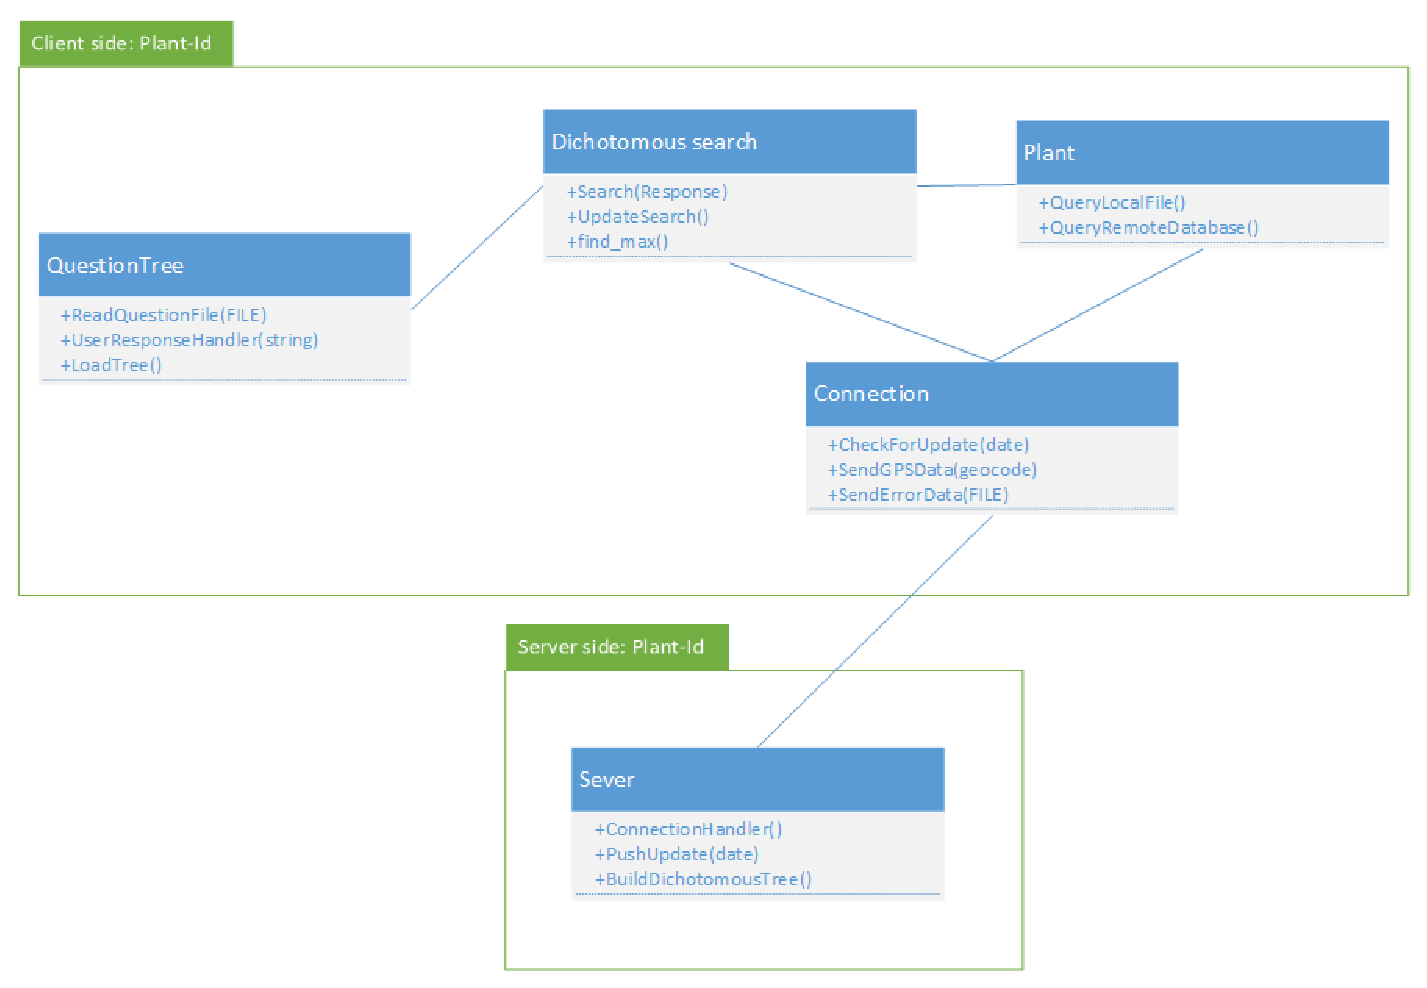
\includegraphics[scale=.48]{UML.eps}\end{center}
\end{frame}
\begin{frame}{UI - Home Screen}
\begin{center}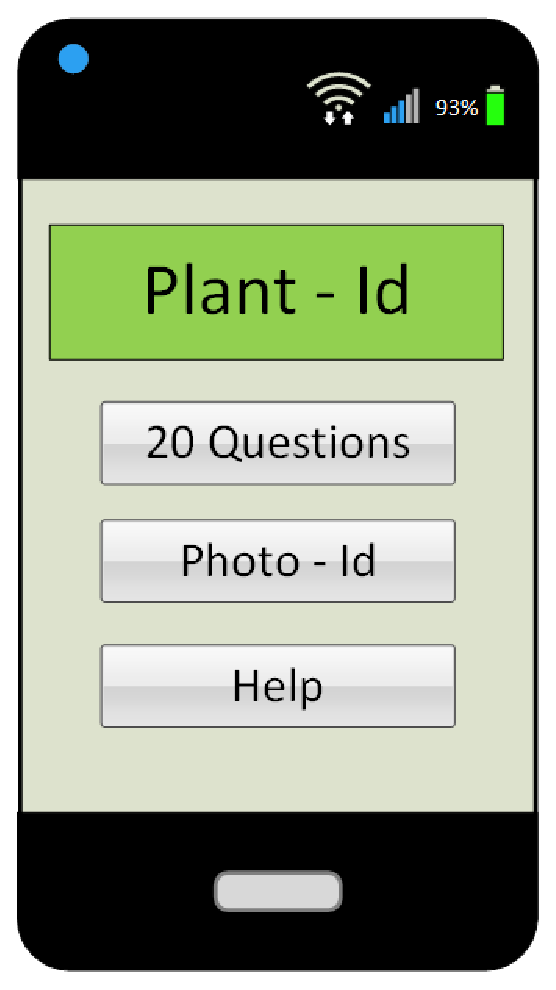
\includegraphics[scale=.5]{HomeScreen.eps}\end{center}
\end{frame}
\begin{frame}{UI - Binary Tree Example}
\begin{center}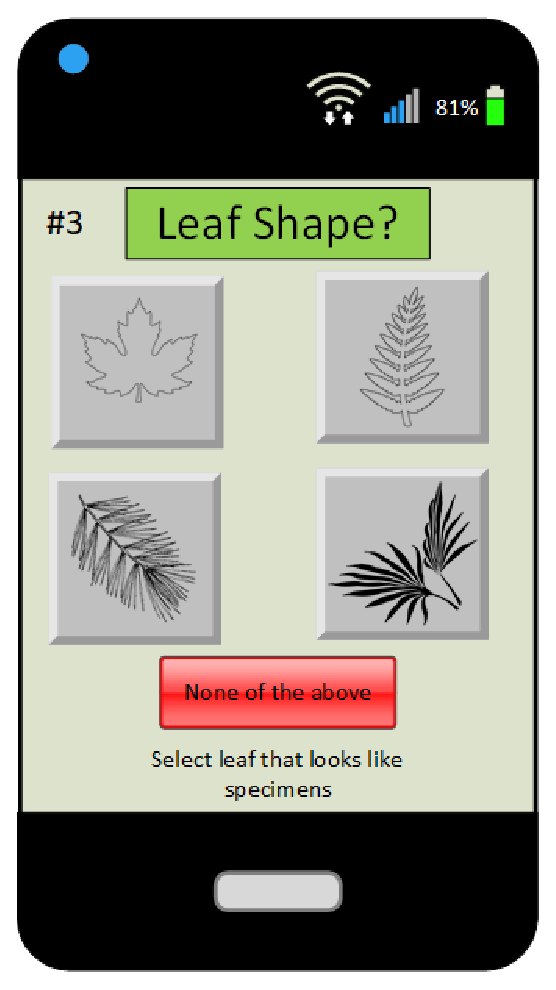
\includegraphics[scale=.5]{20Questions.eps}\end{center}
\end{frame}
\begin{frame}{UI - Image Recognition (if time)}
\begin{center}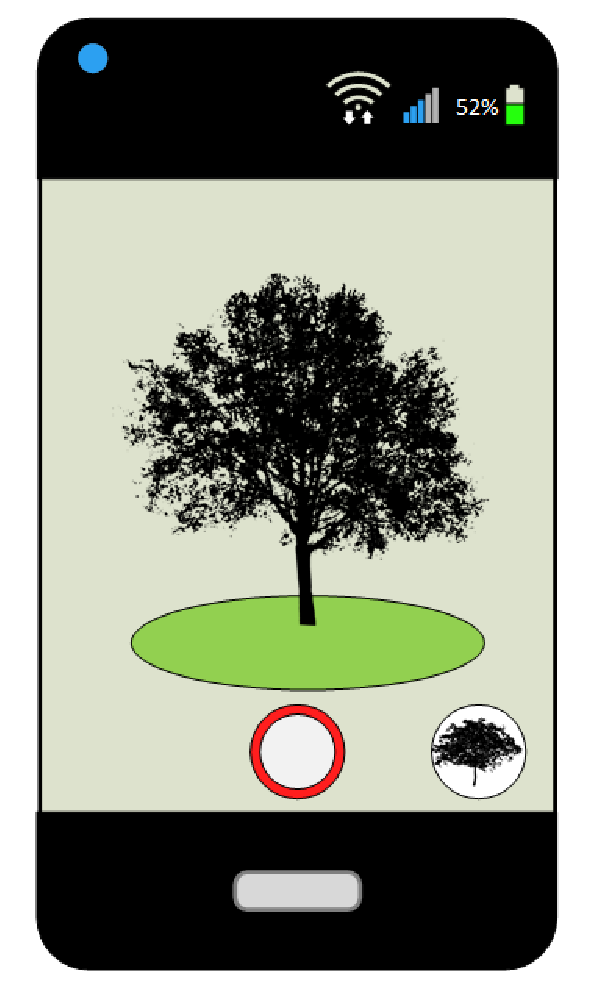
\includegraphics[scale=.5]{Photo-Id.eps}\end{center}
\end{frame}
\begin{frame}{Planning}
Tasks
\begin{itemize}
\item Currently due to time constraints we will be implementing a dichotomous search algorithm.
\item Example of Morse code classification in dichotomous.
\end{itemize}
\end{frame}
\begin{frame}{Risk Analysis}
\begin{itemize}
\item Currently due to time constraints we will be implementing a dichotomous search algorithm.
\newline
\item Biggest risk is time.
\newline
\item Example of Morse code classification in dichotomous search.
\begin{center}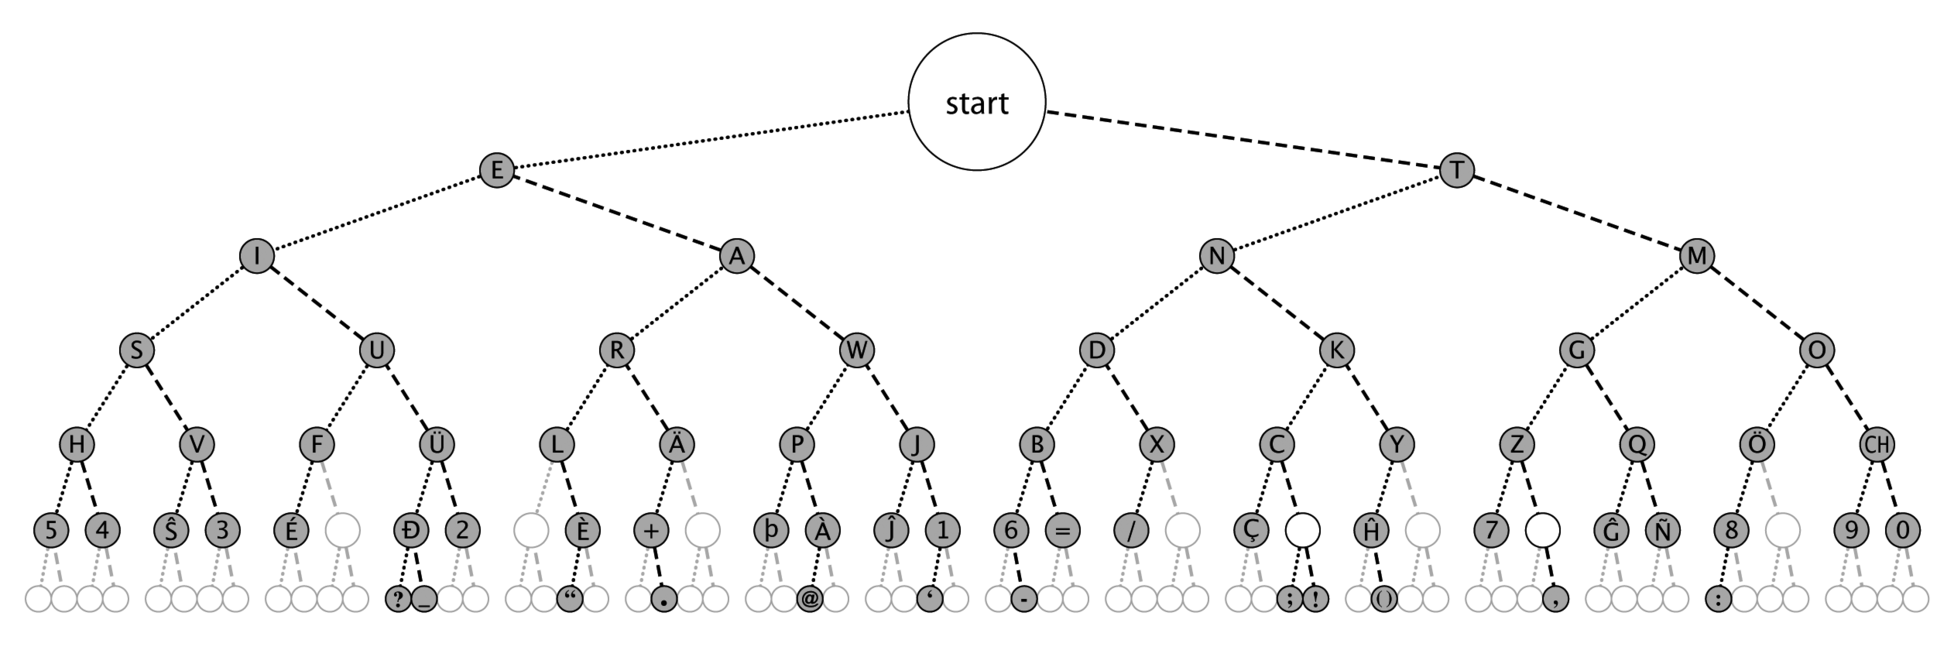
\includegraphics[scale=.3]{Morse_code_tree3.eps}\end{center}
\end{itemize}
\end{frame}
\begin{frame}{Design pattern}
\begin{itemize}
\item At this time we do not plant to implement a design pattern.
\newline
\item The dichotomous tree is simple, adding a design pattern would add more complexity than needed. By design it is simple but useful.
\newline
\item Despite not using a design pattern we will be following standard object oriented programming.
\end{itemize}
\end{frame}
\begin{frame}{Exceptions Handling}
\begin{itemize}
\item If the application fails to display the correct plant, and the user knows this, they can send there response data, and what they think the plant is, back to the development team.
\end{itemize}
\end{frame}
\begin{frame}{Use Case Diagram}
\begin{center}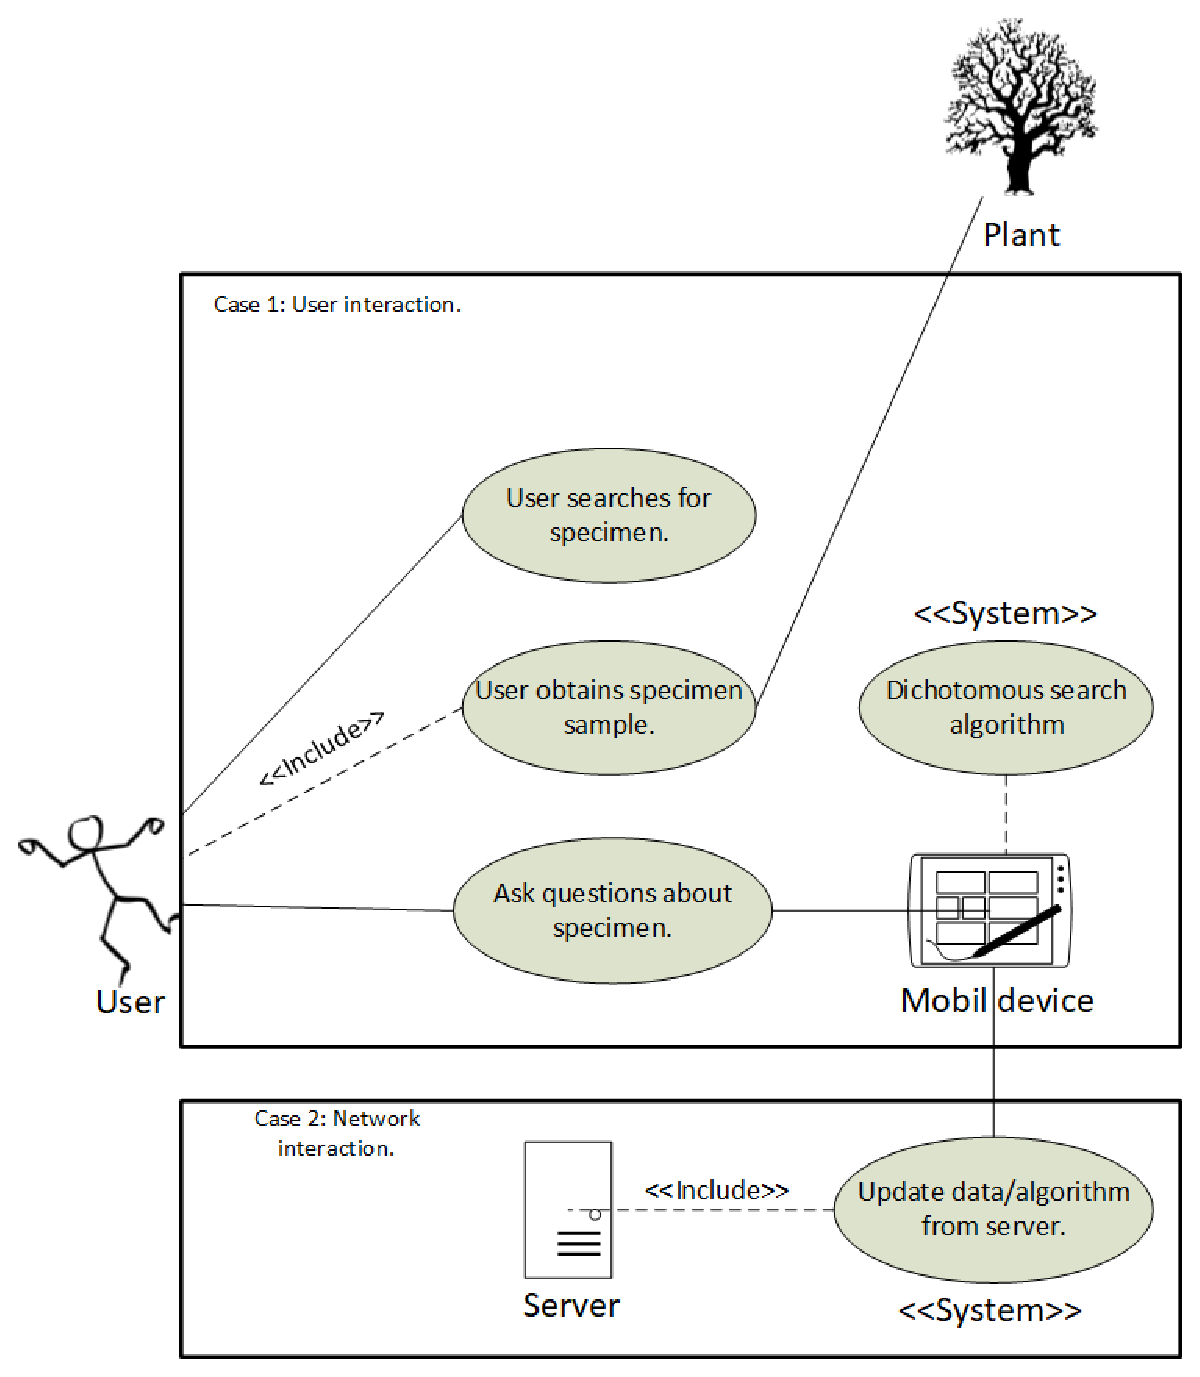
\includegraphics[scale=.35]{search.eps}\end{center}
\end{frame}
\begin{frame}{Sequence Diagram}
\begin{center}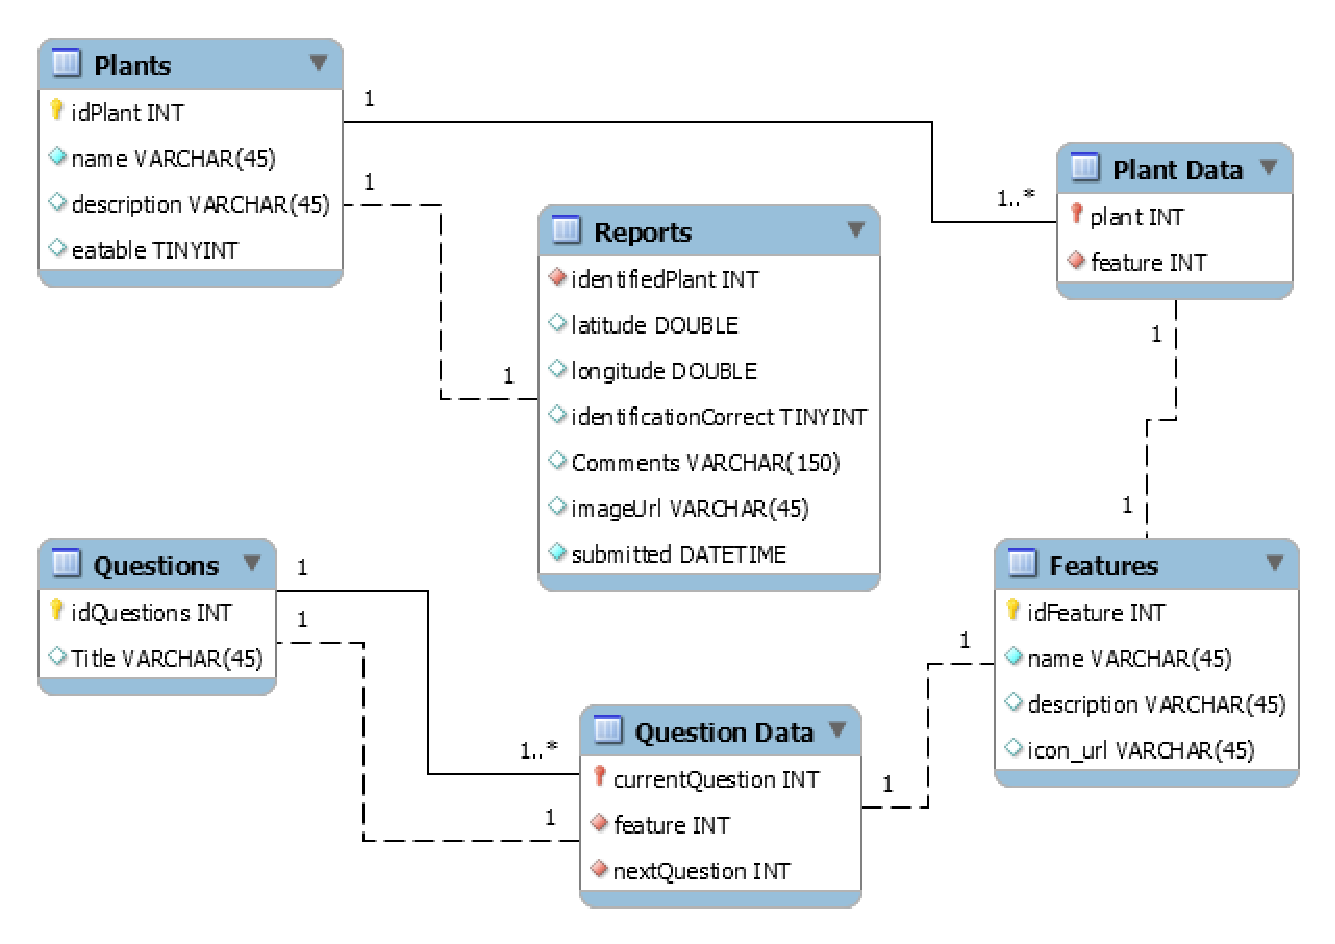
\includegraphics[scale=.5]{DatabaseDesign.eps}\end{center}
\end{frame}
\begin{frame}{Class Diagram}
\begin{center}\includegraphics[scale=.5]{QuestionIdentification.eps}\end{center}
\end{frame}
\begin{frame}{Schedule}
\begin{center}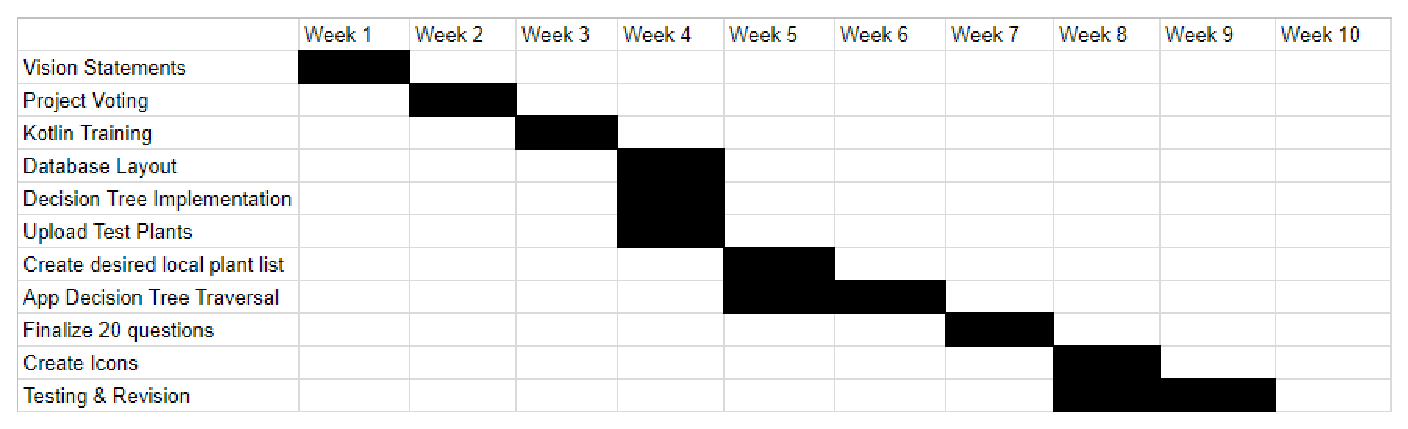
\includegraphics[scale=.48]{schedule.eps}\end{center}
\end{frame}
\end{document}
